\documentclass[aspectratio=169,10pt]{beamer}

\usepackage[utf8]{inputenc}
\usepackage[T1]{fontenc}
\usepackage{lmodern}
\usepackage{amsmath,amssymb}
\usepackage{booktabs,tabularx,array,adjustbox}
\usepackage{tikz,pgfplots}
\usepackage[most]{tcolorbox}
\usepackage{graphicx,xcolor,ragged2e}
\pgfplotsset{compat=1.18}
\usetikzlibrary{arrows.meta,positioning,calc}

% ---------- Palette ----------
\definecolor{DeepNavy}{HTML}{073B4C}
\definecolor{Teal}{HTML}{118AB2}
\definecolor{SoftBlue}{HTML}{E8F4FA}
\definecolor{Orange}{HTML}{F26B21}
\definecolor{SoftOrange}{HTML}{FFF0E6}
\definecolor{Mint}{HTML}{D9F2EC}
\definecolor{Purple}{HTML}{6A4C93}
\definecolor{SoftPurple}{HTML}{F2ECFA}
\definecolor{Gold}{HTML}{F7B801}
\definecolor{SoftGold}{HTML}{FFF7D6}
\definecolor{GrayText}{HTML}{4A5568}
\definecolor{LightLine}{HTML}{D9E2EC}

% ---------- Beamer ----------
\setbeamertemplate{navigation symbols}{}
\setbeamercolor{normal text}{fg=DeepNavy,bg=white}
\setbeamercolor{frametitle}{fg=DeepNavy,bg=white}
\setbeamerfont{frametitle}{size=\Large,series=\bfseries}
\setbeamertemplate{frametitle}{%
  \vspace{0.25em}\insertframetitle\par
  \vspace{-0.25em}\tikz{\draw[Orange,line width=1.15pt] (0,0)--(1.15,0);}\vspace{-0.48em}
}
\setbeamertemplate{footline}{%
\leavevmode\hbox{%
\begin{beamercolorbox}[wd=.46\paperwidth,ht=2.2ex,dp=1ex,leftskip=1em]{}\scriptsize MA25-31017 Pemodelan Komputasi dan Analisis Numerik\end{beamercolorbox}%
\begin{beamercolorbox}[wd=.36\paperwidth,ht=2.2ex,dp=1ex,center]{}\scriptsize Program Studi Matematika ITERA\end{beamercolorbox}%
\begin{beamercolorbox}[wd=.18\paperwidth,ht=2.2ex,dp=1ex,rightskip=1em plus1fil]{}\scriptsize \insertframenumber/\inserttotalframenumber\end{beamercolorbox}}%
}

% ---------- Boxes ----------
\tcbset{enhanced,boxrule=.7pt,arc=2mm,left=2mm,right=2mm,top=1mm,bottom=1mm,fonttitle=\bfseries,before skip=1pt,after skip=1pt}
\newtcolorbox{bluebox}[1][]{colback=SoftBlue,colframe=Teal,title=#1}
\newtcolorbox{orangebox}[1][]{colback=SoftOrange,colframe=Orange,title=#1}
\newtcolorbox{greenbox}[1][]{colback=Mint,colframe=DeepNavy!55!Teal,title=#1}
\newtcolorbox{purplebox}[1][]{colback=SoftPurple,colframe=Purple,title=#1}
\newtcolorbox{goldbox}[1][]{colback=SoftGold,colframe=Gold!80!black,title=#1}
\newcommand{\highlight}[1]{\textcolor{Orange}{\textbf{#1}}}
\newcommand{\smallgray}[1]{\textcolor{GrayText}{\scriptsize #1}}
\newcommand{\excel}[1]{\texttt{\detokenize{#1}}}

\begin{document}

% 1 COVER
\begin{frame}[plain]
\begin{tikzpicture}[remember picture,overlay]
  \fill[SoftBlue] (current page.north west) rectangle ([xshift=.48\paperwidth]current page.south west);
  \fill[white] ([xshift=.48\paperwidth]current page.north west) rectangle (current page.south east);
\end{tikzpicture}
\vspace{0.62cm}
\begin{columns}[T,totalwidth=\textwidth]
\begin{column}{.44\textwidth}
{\fontsize{21}{24}\selectfont\bfseries Pemodelan Komputasi\\dan Analisis Numerik}\par
\vspace{0.12cm}
\tikz{\draw[Orange,line width=1.5pt] (0,0)--(1.9,0);}\par
\vspace{0.15cm}
{\large Kontrak Kuliah dan Pencarian Akar}\par
\vspace{0.50cm}
\small MA25-31017\par
\small Program Studi Matematika\par
\small Institut Teknologi Sumatera\par
\vspace{0.28cm}
\textbf{Dosen Pengampu}\par
Rifky Fauzi\par
Dear Michiko Mutiara Noor
\end{column}
\begin{column}{.52\textwidth}
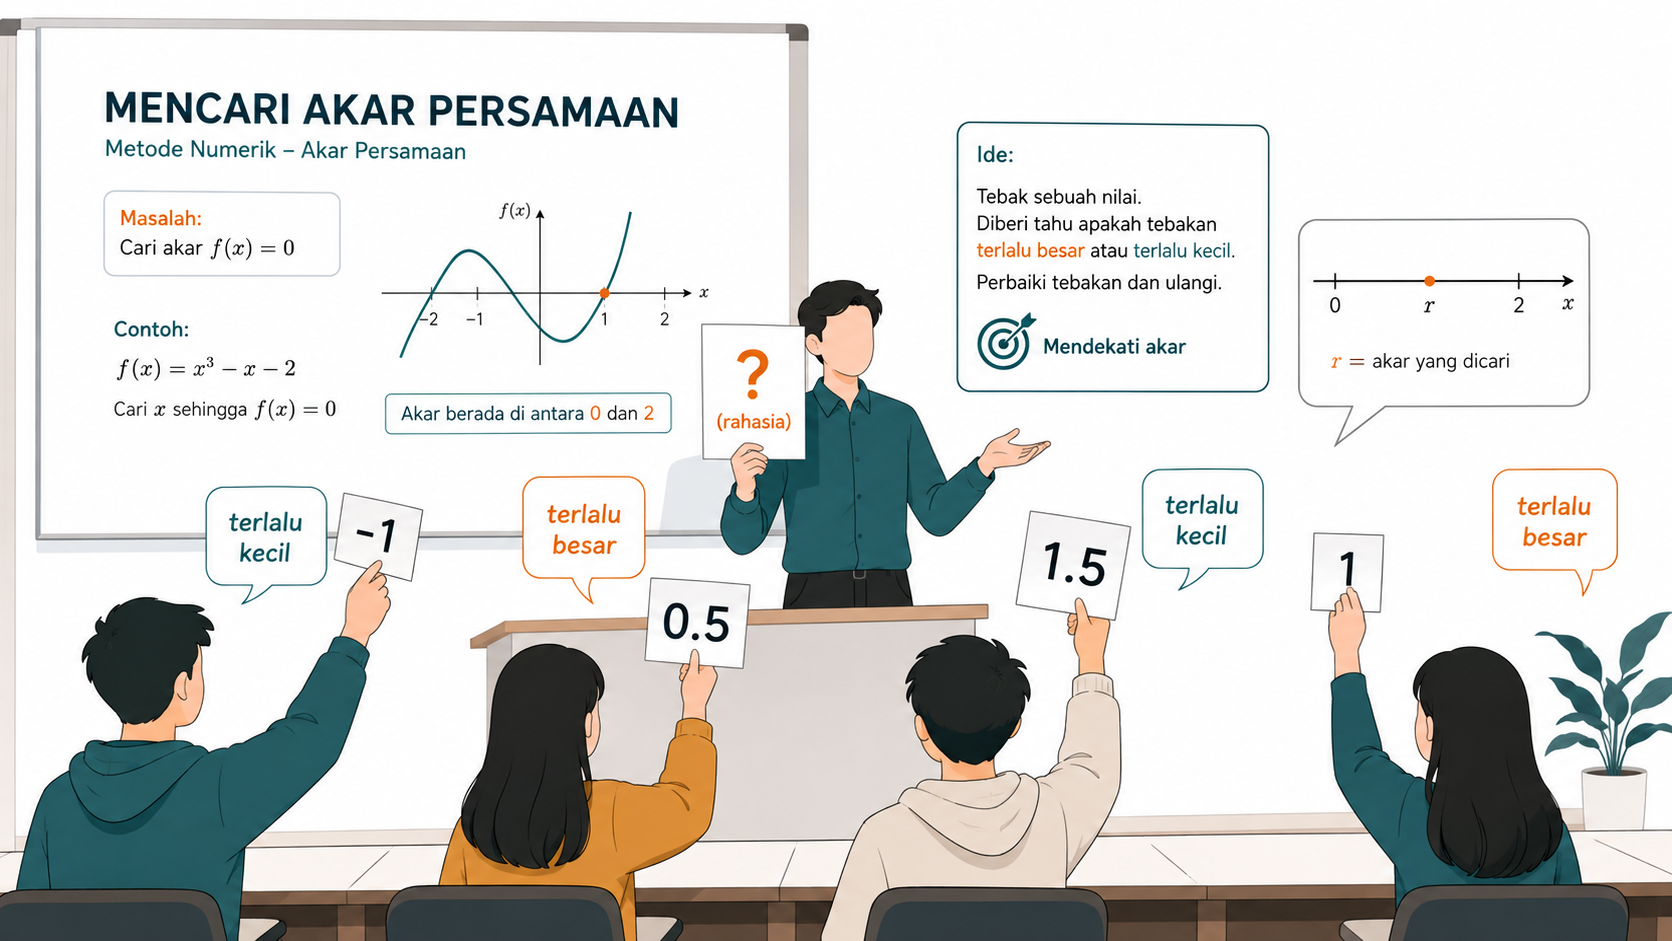
\includegraphics[width=\linewidth,height=.72\textheight,keepaspectratio]{wide_clean_vector_illustration_style_classroom_sli.png}
\end{column}
\end{columns}
\end{frame}

% 2
\begin{frame}{Apa Itu Metode Numerik?}
\small
\begin{columns}[T,totalwidth=\textwidth]
\begin{column}{.50\textwidth}
\begin{bluebox}[Inti menurut Chapra \& Canale]
Metode numerik memformulasikan masalah matematika sehingga penyelesaiannya dapat dilakukan melalui \textbf{operasi aritmetika} yang sistematis dan cocok diimplementasikan dengan komputer.
\end{bluebox}
\begin{orangebox}[Mengapa diperlukan?]
Solusi analitik tetap sangat penting, tetapi banyak masalah nyata bersifat nonlinear, berdimensi tinggi, atau terlalu kompleks untuk memperoleh solusi eksak secara langsung.
\end{orangebox}
\end{column}
\begin{column}{.46\textwidth}
\begin{greenbox}[Bukan hanya menghitung]
Komputer mengambil alih perhitungan berulang sehingga kita dapat memberi perhatian lebih pada:
\begin{enumerate}\setlength\itemsep{2pt}
\item formulasi masalah,
\item pemilihan metode,
\item analisis galat,
\item interpretasi hasil.
\end{enumerate}
\end{greenbox}
\begin{goldbox}[Alur]
\centering \textbf{Model $\rightarrow$ Algoritma $\rightarrow$ Aproksimasi $\rightarrow$ Interpretasi}
\end{goldbox}
\end{column}
\end{columns}
\vfill
\smallgray{Rujukan: Chapra \& Canale, Numerical Methods for Engineers, 7th ed., PT1.1.}
\end{frame}

% 3
\begin{frame}{Mengapa Kita Belajar Metode Numerik?}
\scriptsize
\begin{columns}[T,totalwidth=\textwidth]
\begin{column}{.48\textwidth}
\begin{bluebox}[Masalah yang dapat ditangani]
\begin{tabularx}{\linewidth}{>{\bfseries}p{.31\linewidth} X}
Akar & $f(x)=0$ \\
SPL / SPNL & $F(\mathbf{x})=\mathbf{0}$ \\
Optimisasi & titik terbaik; pada kasus mulus interior sering $\nabla J=\mathbf{0}$ \\
Curve fitting & parameter yang membuat residual/error kecil \\
ODE / PDE & aproksimasi solusi ketika solusi eksak sulit \\
\end{tabularx}
\end{bluebox}
\end{column}
\begin{column}{.48\textwidth}
\begin{orangebox}[Menurut Chapra]
Metode numerik memperluas kemampuan pemecahan masalah untuk sistem besar, nonlinearitas, dan geometri rumit. Pemahaman teori dasar diperlukan agar software tidak dipakai sebagai black box.
\end{orangebox}
\begin{purplebox}[Benang merah MK]
Banyak problem pada akhirnya mencari kondisi tertentu: residual nol, keseimbangan, fixed point, atau minimum error. Karena itu \textbf{iterasi, galat, dan konvergensi} akan berulang sepanjang mata kuliah.
\end{purplebox}
\end{column}
\end{columns}
\vfill
\smallgray{Rujukan: Chapra \& Canale, PT1.1--PT1.2.}
\end{frame}

% 4
\begin{frame}{Kontrak Kuliah: Arah Pembelajaran}
\scriptsize
\begin{columns}[T,totalwidth=\textwidth]
\begin{column}{.50\textwidth}
\begin{bluebox}[Karakter kelas]
\begin{itemize}\setlength\itemsep{2pt}
\item \textbf{Student-centered learning}: mahasiswa aktif, dosen fasilitator.
\item Banyak diskusi, praktik komputasi, telaah jurnal, dan presentasi.
\item Dosen tetap memberi fondasi, arah, standar, serta umpan balik.
\end{itemize}
\end{bluebox}
\begin{greenbox}[Prinsip]
Belajar terbaik adalah mengajar. Kalian akan belajar dengan menjelaskan, mengkritisi, dan saling memperbaiki pemahaman.
\end{greenbox}
\end{column}
\begin{column}{.47\textwidth}
\begin{orangebox}[E-learning]
Quiz dikerjakan di e-learning. Tugas dikumpulkan di e-learning.
\end{orangebox}
\begin{purplebox}[Project]
Luaran akhir: \textbf{program MATLAB} yang dapat dijalankan dan \textbf{draft artikel ilmiah}. Arah lanjut: PKM-AI.
\end{purplebox}
\end{column}
\end{columns}
\end{frame}

% 5
\begin{frame}{Jadwal Kelas dan Aturan Pertemuan}
\scriptsize
\begin{columns}[T,totalwidth=\textwidth]
\begin{column}{.58\textwidth}
\renewcommand{\arraystretch}{1.12}
\begin{tabularx}{\linewidth}{c X X X}
\toprule
Kelas & Kuliah & Praktikum/Jurnal & Ruang\\
\midrule
RA & Jumat 07.30--10.00 & Senin 08.00--10.00 & F306 / Lab\\
RB & Senin 07.30--10.00 & Jumat 08.00--10.00 & F302 / Lab\\
\bottomrule
\end{tabularx}
\end{column}
\begin{column}{.38\textwidth}
\begin{goldbox}[Jika dosen tidak masuk]
Tidak ada pertemuan pengganti. Materi dialihkan ke e-learning dalam mode asynchronous.
\end{goldbox}
\begin{bluebox}[Pertemuan berikutnya]
Kelas diawali diskusi atas materi asynchronous sebelum masuk agenda berikutnya.
\end{bluebox}
\end{column}
\end{columns}
\end{frame}

% 6
\begin{frame}{Komponen Penilaian dan Ujian}
\scriptsize
\begin{columns}[T,totalwidth=\textwidth]
\begin{column}{.58\textwidth}
\renewcommand{\arraystretch}{1.10}
\begin{tabularx}{\linewidth}{X c X}
\toprule
Komponen & Bobot & Pelaksanaan\\
\midrule
Praktik & 15\% & 10 pertemuan\\
Tugas individu & 20\% & e-learning\\
UTS & 10\% & M8: akar + SPL\\
UAS & 10\% & M13: turunan + integral + PDB\\
Quiz & 10\% & e-learning\\
Project & 35\% & MATLAB + draft artikel\\
\bottomrule
\end{tabularx}
\end{column}
\begin{column}{.38\textwidth}
\begin{orangebox}[UTS]
\textbf{Hanya pencarian akar dan SPL}. SPNL dan data-driven model merupakan pengayaan/penghubung menuju pemodelan.
\end{orangebox}
\begin{purplebox}[UAS]
Turunan numerik, integral numerik, dan PDB numerik.
\end{purplebox}
\end{column}
\end{columns}
\end{frame}

% 7
\begin{frame}{Jadwal Pertemuan M1--M8}
\scriptsize
\renewcommand{\arraystretch}{1.13}
\begin{tabularx}{\linewidth}{c X c}
\toprule
M & Agenda & Dosen\\
\midrule
M1 & \textbf{Materi}: pengantar metode numerik, pencarian akar, grafik, Biseksi, Regula Falsi, Titik Tetap, Newton, Secant, galat dan Excel & Rifky\\
M2 & \textbf{Materi}: SPL, SPNL, data-driven model (regresi, regresi nonlinear, pencocokan kurva) & Rifky\\
M3 & \textbf{Bedah jurnal/presentasi}: metode pencarian akar; presenter random, semua siap & Rifky\\
M4 & \textbf{Bedah jurnal/presentasi}: SPL, SPNL, fixed point, optimisasi, data-driven & Rifky\\
M5 & Materi: turunan numerik & Dear\\
M6 & Jurnal/praktikum: turunan numerik & Dear\\
M7 & Materi: integral numerik & Dear\\
M8 & \textbf{UTS: pencarian akar dan SPL} & Rifky\\
\bottomrule
\end{tabularx}
\vspace{1mm}
\begin{goldbox}[Penyesuaian awal]
M1--M2 sengaja sama-sama materi; M3--M4 sama-sama journal sharing untuk menyelesaikan benturan jadwal awal.
\end{goldbox}
\end{frame}

% 8
\begin{frame}{Jadwal Pertemuan M9--M16}
\scriptsize
\renewcommand{\arraystretch}{1.16}
\begin{tabularx}{\linewidth}{c X c}
\toprule
M & Agenda & Dosen\\
\midrule
M9 & Jurnal/praktikum: integral numerik & Dear\\
M10 & Materi: PDB numerik, Euler, Runge-Kutta & Dear\\
M11 & Jurnal/praktikum: model PDB numerik & Dear\\
M12 & Persiapan UAS + praktik ke-10 & Dear\\
M13 & \textbf{UAS: turunan, integral, PDB numerik} & Dear\\
M14 & Project 1: formulasi, rancangan MATLAB, progress & Rifky\\
M15 & Project 2: implementasi, verification/validation, progress & Rifky\\
M16 & Final project: demo MATLAB + draft artikel + presentasi akhir & Rifky\\
\bottomrule
\end{tabularx}
\begin{purplebox}[Project meeting]
Setiap pertemuan project memuat presentasi singkat: \textbf{capaian, kendala, dan rencana tindak lanjut}.
\end{purplebox}
\end{frame}

% 9 GAME
\begin{frame}{Aktivitas Awal: Permainan Tebak Angka}
\scriptsize
\begin{columns}[T,totalwidth=\textwidth]
\begin{column}{.49\textwidth}
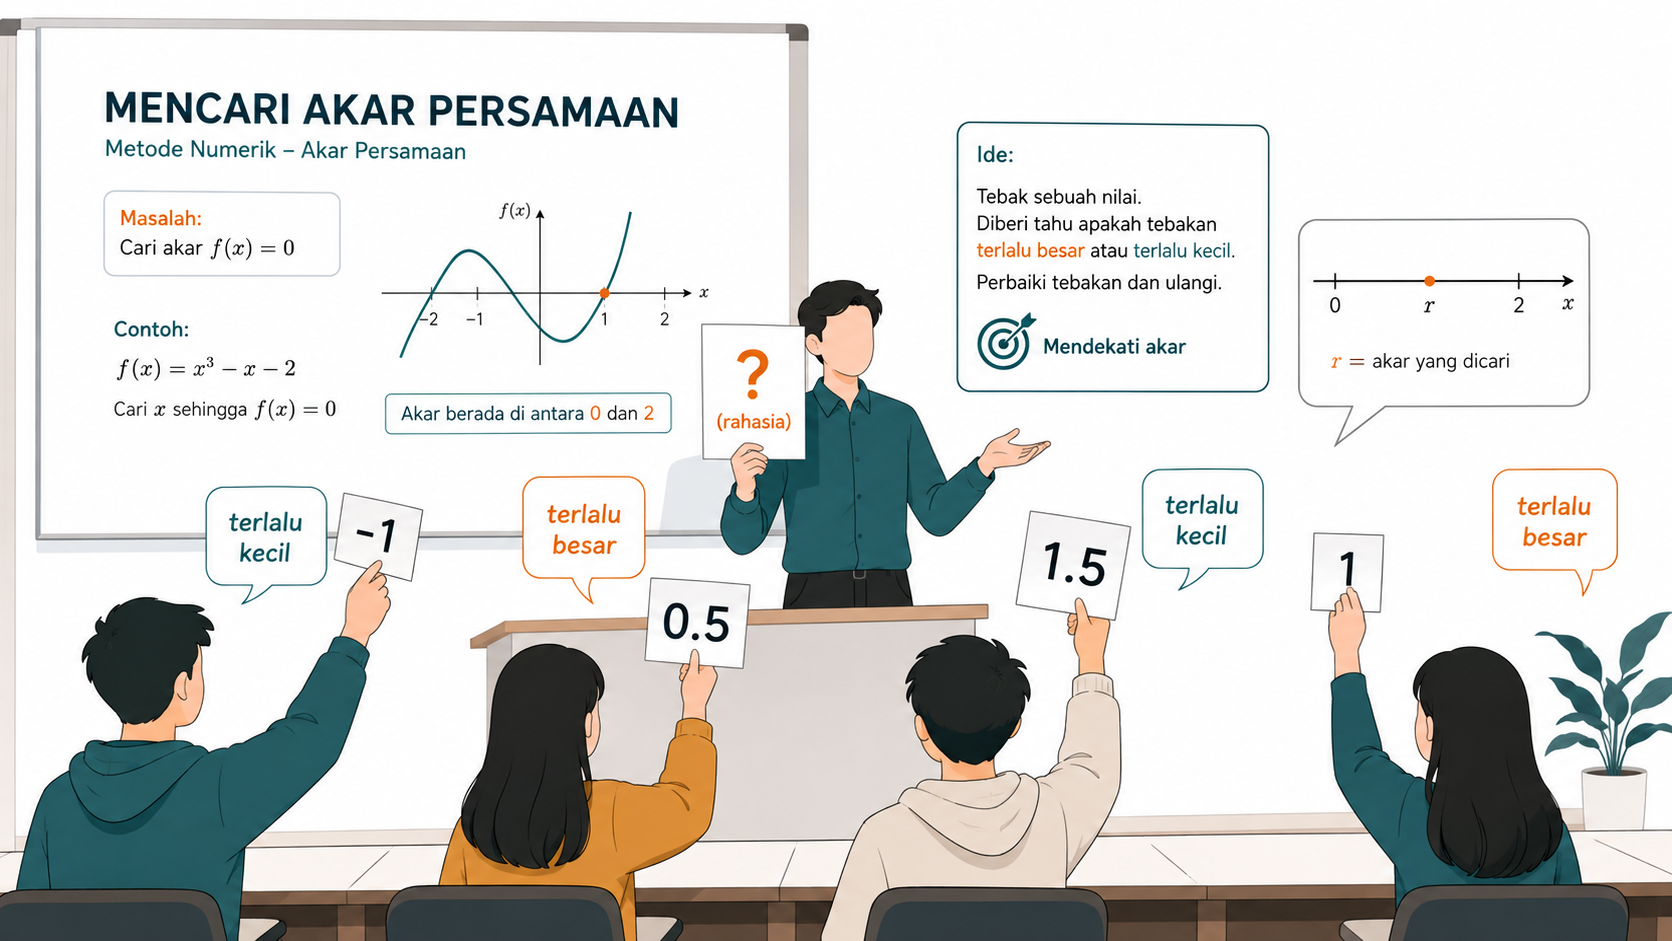
\includegraphics[width=\linewidth,height=.62\textheight,keepaspectratio]{wide_clean_vector_illustration_style_classroom_sli.png}
\end{column}
\begin{column}{.47\textwidth}
\begin{bluebox}[Aturan main]
Dosen memilih satu angka rahasia. Mahasiswa menebak. Dosen hanya menjawab \highlight{terlalu besar} atau \highlight{terlalu kecil}.
\end{bluebox}
\begin{enumerate}\setlength\itemsep{5pt}
\item Tebak angka.
\item Dapat umpan balik.
\item Persempit kemungkinan.
\item Ulangi sampai cukup dekat.
\item Yang benar memilih angka berikutnya.
\end{enumerate}
\begin{orangebox}[]
Miniatur metode iteratif: \textbf{tebak, evaluasi, perbaiki}. Semua mahasiswa berpartisipasi.
\end{orangebox}
\end{column}
\end{columns}
\end{frame}

% 10
\begin{frame}{Prinsip Utama Pencarian Akar}
\small
\begin{bluebox}[Masalah]
Cari nilai \(x\) yang membuat
\[
f(x)=0.
\]
Akar adalah titik ketika residual fungsi menjadi nol.
\end{bluebox}
\begin{columns}[T,totalwidth=\textwidth]
\begin{column}{.48\textwidth}
\begin{greenbox}[Satu variabel]
Contoh:
\[
f(x)=x^3-x-1.
\]
Kita mencari lokasi ketika grafik memotong sumbu-\(x\).
\end{greenbox}
\end{column}
\begin{column}{.48\textwidth}
\begin{orangebox}[Dimensi lebih tinggi]
\[
F(\mathbf{x})=\mathbf{0}.
\]
Ide yang sama muncul pada SPNL, equilibrium, optimisasi (gradien nol), fitting, dan banyak algoritma AI/data-driven.
\end{orangebox}
\end{column}
\end{columns}
\end{frame}

% 11 GRAPHING
\begin{frame}{Graphing Method: Lihat Dulu, Baru Hitung}
\scriptsize
\begin{columns}[T,totalwidth=\textwidth]
\begin{column}{.56\textwidth}
\begin{tikzpicture}
\begin{axis}[width=\linewidth,height=.64\textheight,axis lines=middle,xmin=.6,xmax=1.7,ymin=-1.5,ymax=2.2,grid=both,grid style={LightLine!55},xlabel={$x$},ylabel={$f(x)$},xtick={1,1.5},ytick={-1,0,.875}]
\addplot[DeepNavy,very thick,domain=.6:1.7,samples=150]{x^3-x-1};
\addplot[only marks,mark=*,Orange] coordinates {(1,-1) (1.5,.875)};
\end{axis}
\end{tikzpicture}
\end{column}
\begin{column}{.40\textwidth}
\begin{bluebox}[Contoh grafik]
\[
f(1)=-1,\qquad f(1.5)=0.875.
\]
Karena
\[
f(1)f(1.5)<0,
\]
ada perubahan tanda, sehingga akar terkurung di antara 1 dan 1.5.
\end{bluebox}
\begin{goldbox}[Kegunaan grafik]
Memahami bentuk fungsi dan memilih tebakan/interval awal yang masuk akal.
\end{goldbox}
\end{column}
\end{columns}
\end{frame}

% 12
\begin{frame}{Biseksi: Bahasa Formal dari Permainan Tebak Angka}
\scriptsize
\begin{columns}[T,totalwidth=\textwidth]
\begin{column}{.49\textwidth}
\begin{bluebox}[1. Pilih interval awal]
\(a\) dan \(b\) boleh dipilih bebas selama
\[
f(a)f(b)<0.
\]
Ini memastikan perubahan tanda pada interval.
\end{bluebox}
\begin{orangebox}[2. Hitung titik tengah]
Bukan menebak secara bebas:
\[
x_r=\frac{a+b}{2}.
\]
\end{orangebox}
\end{column}
\begin{column}{.47\textwidth}
\begin{greenbox}[3. Pilih setengah interval]
Jika \(f(a)f(x_r)<0\), perubahan tanda ada antara \(a\) dan \(x_r\), maka pilih
\[
[a,x_r].
\]
Jika \(f(a)f(x_r)>0\), pilih
\[
[x_r,b].
\]
\end{greenbox}
\begin{goldbox}[4. Ulangi]
Terus persempit interval sampai galat memenuhi toleransi.
\end{goldbox}
\end{column}
\end{columns}
\end{frame}

% 13 ERROR CONCEPT
\begin{frame}{Mengapa Metode Numerik Selalu Berbicara tentang Galat?}
\small
\begin{columns}[T,totalwidth=\textwidth]
\begin{column}{.50\textwidth}
\begin{bluebox}[Numerik = hampiran]
Metode numerik umumnya membangun \textbf{aproksimasi}. Jika hasilnya ``hampir'' sama dengan solusi ideal, secara alami ada selisih yang harus diukur.
\end{bluebox}
\begin{orangebox}[Pertanyaannya bukan ``ada galat atau tidak?'']
Pertanyaan yang lebih tepat: \textbf{seberapa besar galatnya dan apakah sudah cukup kecil untuk kebutuhan kita?}
\end{orangebox}
\end{column}
\begin{column}{.46\textwidth}
\begin{greenbox}[Sumber galat]
\begin{itemize}\setlength\itemsep{2pt}
\item truncation error,
\item round-off error,
\item iterative error,
\item ketidakpastian data/model.
\end{itemize}
\end{greenbox}
\begin{goldbox}[Pelajaran]
Hasil numerik tanpa informasi galat atau konvergensi belum cukup meyakinkan.
\end{goldbox}
\end{column}
\end{columns}
\vfill
\smallgray{Chapra menempatkan error analysis sebagai bagian fundamental dari penggunaan metode numerik.}
\end{frame}

% 14 ERROR FORMULAS
\begin{frame}{Galat, Galat Relatif, dan Toleransi}
\scriptsize
\begin{columns}[T,totalwidth=\textwidth]
\begin{column}{.50\textwidth}
\begin{bluebox}[Jika nilai sebenarnya diketahui]
Galat absolut:
\[
E_t=\left|x_{\rm true}-x_{\rm approx}\right|.
\]
Galat relatif sebenarnya:
\[
\varepsilon_t=\left|\frac{x_{\rm true}-x_{\rm approx}}{x_{\rm true}}\right|100\%.
\]
\end{bluebox}
\end{column}
\begin{column}{.46\textwidth}
\begin{orangebox}[Jika nilai sebenarnya tidak diketahui]
Untuk iterasi:
\[
\varepsilon_a=\left|\frac{x^{(k)}-x^{(k-1)}}{x^{(k)}}\right|100\%.
\]
\end{orangebox}
\begin{goldbox}[Stopping criterion]
Dengan toleransi \(\varepsilon_s\), iterasi dapat dihentikan jika
\[
\varepsilon_a<\varepsilon_s,
\]
serta selalu siapkan iterasi maksimum.
\end{goldbox}
\end{column}
\end{columns}
\vfill
\smallgray{Chapra \& Canale, Ch. 3: true relative error, approximate relative error, acceptable error.}
\end{frame}

% 15 BISECTION TABLE
\begin{frame}{Latihan Kelas: Biseksi untuk $f(x)=x^3-x-1$}
\tiny
\begin{bluebox}[Aktivitas]
Gunakan interval awal \([1,1.5]\). Lengkapi titik-titik sampai toleransi tercapai.
\end{bluebox}
\renewcommand{\arraystretch}{1.08}
\begin{adjustbox}{max width=\linewidth,center}
\begin{tabular}{c c c c c c c c c c}
\toprule
iterasi & $a$ & $b$ & $f(a)$ & $f(b)$ & $x_r$ & $f(x_r)$ & $f(a)f(x_r)$ & lokasi & $\varepsilon_a$\\
\midrule
1 & 1.000 & 1.500 & -1.000 & 0.875 & 1.250 & -0.2969 & $0.2969>0$ & $[x_r,b]$ & --\\
2 & 1.250 & 1.500 & -0.2969 & 0.875 & 1.375 & 0.2246 & $-0.0667<0$ & $[a,x_r]$ & 9.09\%\\
3 & $\cdots$ & $\cdots$ & $\cdots$ & $\cdots$ & $\cdots$ & $\cdots$ & $\cdots$ & $\cdots$ & $\cdots$\\
4 & $\cdots$ & $\cdots$ & $\cdots$ & $\cdots$ & $\cdots$ & $\cdots$ & $\cdots$ & $\cdots$ & $\cdots$\\
5 & $\cdots$ & $\cdots$ & $\cdots$ & $\cdots$ & $\cdots$ & $\cdots$ & $\cdots$ & $\cdots$ & $\cdots$\\
\bottomrule
\end{tabular}
\end{adjustbox}
\end{frame}

% 16 EXCEL
\begin{frame}{Demo Excel: Dari Tabel ke Algoritma}
\tiny
\begin{columns}[T,totalwidth=\textwidth]
\begin{column}{.48\textwidth}
\begin{bluebox}[Kolom]
A: iterasi, B: $a$, C: $b$, D: $f(a)$, E: $f(b)$, F: $x_r$, G: $f(x_r)$, H: $f(a)f(x_r)$, I: lokasi, J: $\varepsilon_a$.
\end{bluebox}
\begin{tabularx}{\linewidth}{p{.13\linewidth} X}
\toprule
Cell & Formula baris 2\\
\midrule
D2 & \excel{=B2^3-B2-1}\\
E2 & \excel{=C2^3-C2-1}\\
F2 & \excel{=(B2+C2)/2}\\
G2 & \excel{=F2^3-F2-1}\\
H2 & \excel{=D2*G2}\\
I2 & \excel{=IF(H2<0,"[a,xr]","[xr,b]")}\\
J2 & \excel{="-"}\\
\bottomrule
\end{tabularx}
\end{column}
\begin{column}{.48\textwidth}
\begin{orangebox}[Baris selanjutnya]
Interval baru mengikuti tanda kolom H.
\end{orangebox}
\begin{tabularx}{\linewidth}{p{.13\linewidth} X}
\toprule
Cell & Formula baris 3\\
\midrule
B3 & \excel{=IF(H2<0,B2,F2)}\\
C3 & \excel{=IF(H2<0,F2,C2)}\\
D3 & \excel{=B3^3-B3-1}\\
E3 & \excel{=C3^3-C3-1}\\
F3 & \excel{=(B3+C3)/2}\\
G3 & \excel{=F3^3-F3-1}\\
H3 & \excel{=D3*G3}\\
J3 & \excel{=ABS((F3-F2)/F3)*100}\\
\bottomrule
\end{tabularx}
\end{column}
\end{columns}
\end{frame}

% 17 REGULA GRAPH
\begin{frame}{Regula Falsi: Akar Garis Secant Menjadi Kandidat Baru}
\scriptsize
\begin{columns}[T,totalwidth=\textwidth]
\begin{column}{.55\textwidth}
\begin{tikzpicture}
\begin{axis}[width=\linewidth,height=.64\textheight,axis lines=middle,xmin=.9,xmax=1.58,ymin=-1.2,ymax=1.15,grid=both,grid style={LightLine!55},xlabel={$x$},ylabel={$f(x)$},xtick={1,1.2667,1.5},xticklabels={$a$,$x_r$,$b$}]
\addplot[DeepNavy,very thick,domain=.9:1.58,samples=180]{x^3-x-1};
\addplot[Orange,very thick,domain=.98:1.53]{3.75*x-4.75};
\addplot[only marks,mark=*,Teal] coordinates {(1,-1) (1.5,.875)};
\addplot[only marks,mark=*,Orange] coordinates {(1.2666667,0)};
\node[font=\scriptsize,Orange,anchor=south east] at (axis cs:1.47,.75) {garis melalui $(a,f(a))$ dan $(b,f(b))$};
\end{axis}
\end{tikzpicture}
\end{column}
\begin{column}{.41\textwidth}
\begin{bluebox}[Konstruksi]
Pilih \(a,b\) dengan \(f(a)f(b)<0\). Bangun garis melalui dua titik ujung. \textbf{Titik potong garis itu dengan sumbu-\(x\)} adalah kandidat \(x_r\).
\end{bluebox}
\begin{orangebox}[Formula]
\[
x_r=b-f(b)\frac{b-a}{f(b)-f(a)}.
\]
\end{orangebox}
\begin{greenbox}[Contoh]
\(a=1\), \(b=1.5\) memberi \(x_r=1.266667\).
\end{greenbox}
\end{column}
\end{columns}
\end{frame}

% 18 REGULA TABLE
\begin{frame}{Regula Falsi: Enam Iterasi Pertama}
\tiny
\renewcommand{\arraystretch}{1.08}
\begin{adjustbox}{max width=\linewidth,center}
\begin{tabular}{c c c c c c c c c}
\toprule
$i$ & $a$ & $b$ & $f(a)$ & $f(b)$ & $x_r$ & $f(x_r)$ & interval baru & $\varepsilon_a$\\
\midrule
1 & 1.0000 & 1.5000 & -1.0000 & 0.8750 & 1.266667 & -0.234370 & $[x_r,b]$ & --\\
2 & 1.2667 & 1.5000 & -0.2344 & 0.8750 & 1.315962 & -0.037038 & $[x_r,b]$ & 3.7459\%\\
3 & 1.3160 & 1.5000 & -0.0370 & 0.8750 & 1.323436 & -0.005462 & $[x_r,b]$ & 0.5647\%\\
4 & 1.3234 & 1.5000 & -0.0055 & 0.8750 & 1.324531 & -0.000797 & $[x_r,b]$ & 0.08270\%\\
5 & 1.3245 & 1.5000 & -0.0008 & 0.8750 & 1.324691 & -0.000116 & $[x_r,b]$ & 0.01206\%\\
6 & 1.3247 & 1.5000 & -0.0001 & 0.8750 & 1.324714 & -0.000017 & $[x_r,b]$ & 0.001757\%\\
\bottomrule
\end{tabular}
\end{adjustbox}
\begin{bluebox}[Perhatikan]
Pada contoh ini \(b\) relatif ``terkunci'', sedangkan \(a\) bergerak mendekati akar. Ini salah satu alasan False Position dapat lebih lambat pada bentuk kurva tertentu.
\end{bluebox}
\end{frame}

% 19 REGULA ERROR
\begin{frame}{Regula Falsi: Plot Galat Aproksimasi}
\small
\begin{columns}[T,totalwidth=\textwidth]
\begin{column}{.66\textwidth}

\begin{tikzpicture}
\begin{axis}[ymode=log,width=\linewidth,height=.65\textheight,xlabel={Iterasi},ylabel={$\varepsilon_a$ (\%)},xmin=1.8,xmax=6.2,xtick={2,3,4,5,6},grid=both,grid style={LightLine!55}]
\addplot[very thick,Orange,mark=*] coordinates {(2,3.74593) (3,.564733) (4,.0827022) (5,.0120586) (6,.00175712)};
\end{axis}
\end{tikzpicture}
\end{column}
\begin{column}{.29\textwidth}
\begin{orangebox}[Interpretasi]
Galat turun konsisten beberapa orde besaran.
\end{orangebox}
\begin{goldbox}[Bandingkan nanti]
Apakah penurunan ini lebih cepat atau lebih lambat daripada Titik Tetap dan Newton?
\end{goldbox}
\end{column}
\end{columns}
\end{frame}

% 20 FIXED POINT
\begin{frame}{Metode Titik Tetap: $f(x)=e^{-x}-x=0$}
\scriptsize
\begin{columns}[T,totalwidth=\textwidth]
\begin{column}{.47\textwidth}
\begin{bluebox}[Susun ulang]
\[
e^{-x}-x=0
\quad\Longleftrightarrow\quad
x=e^{-x}.
\]
Definisikan
\[
g(x)=e^{-x},\qquad x_{i+1}=g(x_i).
\]
\end{bluebox}
\begin{greenbox}[Fixed point]
Jika \(x_i\to x^*\), maka \(x^*=g(x^*)\), sehingga \(f(x^*)=0\).
\end{greenbox}
\end{column}
\begin{column}{.49\textwidth}
\begin{tikzpicture}
\begin{axis}[width=\linewidth,height=.64\textheight,axis lines=middle,xmin=0,xmax=1.05,ymin=0,ymax=1.05,grid=both,grid style={LightLine!45},xlabel={$x$},ylabel={$y$}]
\addplot[domain=0:1.05,samples=120,thick,Teal]{exp(-x)};
\addplot[domain=0:1.05,thick,DeepNavy]{x};
\draw[Orange,thick] (axis cs:0,0)--(axis cs:0,1)--(axis cs:1,1)--(axis cs:1,.367879)--(axis cs:.367879,.367879)--(axis cs:.367879,.692201)--(axis cs:.692201,.692201)--(axis cs:.692201,.500474)--(axis cs:.500474,.500474)--(axis cs:.500474,.606244);
\node[font=\scriptsize,Teal] at (axis cs:.78,.40) {$y=e^{-x}$};
\node[font=\scriptsize,DeepNavy] at (axis cs:.82,.92) {$y=x$};
\end{axis}
\end{tikzpicture}
\end{column}
\end{columns}
\end{frame}

% 21 FIXED CONVERGENCE
\begin{frame}{Kapan Iterasi Titik Tetap Konvergen?}
\scriptsize
\begin{columns}[T,totalwidth=\textwidth]
\begin{column}{.52\textwidth}
\begin{bluebox}[Syarat praktis lokal]
Untuk \(x_{k+1}=g(x_k)\), indikator penting adalah
\[
\left|g'(x)\right|<1
\]
di sekitar fixed point. Jika magnitudo kemiringan lebih kecil dari satu, galat cenderung teredam.
\end{bluebox}
\begin{orangebox}[Contoh fungsi iterasi]
\[
g'(x)=-e^{-x}.
\]
Pada \(x^*\approx0.567143\):
\[
\left|g'(x^*)\right|\approx0.567143<1.
\]
\end{orangebox}
\end{column}
\begin{column}{.44\textwidth}
\begin{greenbox}[Catatan Chapra]
Kurva fungsi iterasi yang relatif landai di sekitar perpotongan dengan \(y=x\) mendukung konvergensi fixed-point.
\end{greenbox}
\begin{goldbox}[Hati-hati]
Penyusunan \(g(x)\) tidak unik. Transformasi berbeda dapat menghasilkan iterasi yang konvergen atau divergen.
\end{goldbox}
\end{column}
\end{columns}
\end{frame}

% 22 FIXED TABLE
\begin{frame}{Titik Tetap: Enam Langkah Awal}
\scriptsize
\renewcommand{\arraystretch}{1.10}
\begin{columns}[T,totalwidth=\textwidth]
\begin{column}{.60\textwidth}
\begin{tabular}{c c c c}
\toprule
$i$ & $x_i$ & $x_{i+1}=e^{-x_i}$ & $\varepsilon_a$\\
\midrule
0 & 0.000000 & 1.000000 & --\\
1 & 1.000000 & 0.367879 & 171.828\%\\
2 & 0.367879 & 0.692201 & 46.854\%\\
3 & 0.692201 & 0.500474 & 38.309\%\\
4 & 0.500474 & 0.606244 & 17.447\%\\
5 & 0.606244 & 0.545396 & 11.157\%\\
6 & 0.545396 & 0.579612 & 5.903\%\\
\bottomrule
\end{tabular}
\end{column}
\begin{column}{.35\textwidth}
\begin{bluebox}[Pola]
Nilai berosilasi di sekitar akar, tetapi amplitudo osilasinya mengecil.
\end{bluebox}
\begin{orangebox}[Target]
Teruskan sampai \(\varepsilon_a<\varepsilon_s\).
\end{orangebox}
\end{column}
\end{columns}
\end{frame}

% 23 FIXED ERROR
\begin{frame}{Titik Tetap: Plot Galat Aproksimasi}
\small
\begin{columns}[T,totalwidth=\textwidth]
\begin{column}{.66\textwidth}

\begin{tikzpicture}
\begin{axis}[ymode=log,width=\linewidth,height=.65\textheight,xlabel={Iterasi},ylabel={$\varepsilon_a$ (\%)},xmin=.7,xmax=6.3,xtick={1,2,3,4,5,6},grid=both,grid style={LightLine!55}]
\addplot[very thick,Teal,mark=*] coordinates {(1,171.828) (2,46.8536) (3,38.3091) (4,17.4468) (5,11.1566) (6,5.903)};
\end{axis}
\end{tikzpicture}
\end{column}
\begin{column}{.29\textwidth}
\begin{greenbox}[Interpretasi]
Konvergen, tetapi relatif lambat untuk contoh ini.
\end{greenbox}
\begin{goldbox}[Kelebihan]
Sederhana dan tidak memerlukan turunan.
\end{goldbox}
\end{column}
\end{columns}
\end{frame}

% 24 NEWTON GRAPH
\begin{frame}{Newton-Raphson: Akar Garis Singgung Menjadi Kandidat Baru}
\scriptsize
\begin{columns}[T,totalwidth=\textwidth]
\begin{column}{.55\textwidth}
\begin{tikzpicture}
\begin{axis}[width=\linewidth,height=.64\textheight,axis lines=middle,xmin=-.05,xmax=.9,ymin=-.35,ymax=1.10,grid=both,grid style={LightLine!45},xlabel={$x$},ylabel={$f(x)$}]
\addplot[domain=-.05:.9,samples=180,thick,DeepNavy]{exp(-x)-x};
\addplot[domain=-.02:.65,thick,Orange]{1-2*x};
\addplot[domain=.38:.72,thick,Purple]{.10653066-1.60653066*(x-.5)};
\addplot[only marks,mark=*,Orange] coordinates {(0,1) (.5,0)};
\addplot[only marks,mark=*,Purple] coordinates {(.5,.10653066) (.566311,0)};
\node[font=\scriptsize,Orange] at (axis cs:.18,.82) {tangen di $x_0$};
\node[font=\scriptsize,Purple] at (axis cs:.68,-.13) {tangen di $x_1$};
\end{axis}
\end{tikzpicture}
\end{column}
\begin{column}{.41\textwidth}
\begin{bluebox}[Ide]
Di \(x_i\), kurva didekati oleh garis singgung. \textbf{Akar garis singgung} menjadi \(x_{i+1}\).
\end{bluebox}
\begin{orangebox}[Formula]
\[
x_{i+1}=x_i-\frac{f(x_i)}{f'(x_i)}.
\]
\end{orangebox}
\begin{greenbox}[Mirip Regula Falsi]
Keduanya mencari akar dari garis linear. Regula Falsi memakai dua titik; Newton memakai satu titik dan turunan.
\end{greenbox}
\end{column}
\end{columns}
\end{frame}

% 25 NEWTON TABLE
\begin{frame}{Newton-Raphson untuk $f(x)=e^{-x}-x$}
\tiny
\[
f'(x)=-e^{-x}-1,\qquad x_{i+1}=x_i-\frac{e^{-x_i}-x_i}{-e^{-x_i}-1}.
\]
\renewcommand{\arraystretch}{1.08}
\begin{adjustbox}{max width=\linewidth,center}
\begin{tabular}{c c c c c c}
\toprule
$i$ & $x_i$ & $f(x_i)$ & $f'(x_i)$ & $x_{i+1}$ & $\varepsilon_a$\\
\midrule
0 & 0.000000 & 1.000000 & -2.000000 & 0.500000 & 100.000\%\\
1 & 0.500000 & 0.106531 & -1.606531 & 0.566311 & 11.7093\%\\
2 & 0.566311 & 0.001305 & -1.567616 & 0.567143 & 0.146729\%\\
3 & 0.567143 & $1.965\times10^{-7}$ & -1.567143 & 0.56714329 & $2.211\times10^{-5}$\%\\
4 & 0.56714329 & $4.44\times10^{-15}$ & -1.56714329 & 0.56714329 & $5.09\times10^{-13}$\%\\
\bottomrule
\end{tabular}
\end{adjustbox}
\begin{greenbox}[Konvergensi]
Setelah tebakan memasuki daerah yang baik, Newton-Raphson turun sangat cepat menuju akar.
\end{greenbox}
\end{frame}

% 26 NEWTON ERROR
\begin{frame}{Newton-Raphson: Plot Galat Aproksimasi}
\small
\begin{columns}[T,totalwidth=\textwidth]
\begin{column}{.66\textwidth}
\begin{tikzpicture}
\begin{axis}[ymode=log,width=\linewidth,height=.65\textheight,xlabel={Iterasi},ylabel={$\varepsilon_a$ (\%)},xmin=-.2,xmax=4.2,xtick={0,1,2,3,4},ymin=1e-13,ymax=200,grid=both,grid style={LightLine!55}]
\addplot[very thick,Purple,mark=*] coordinates {(0,100) (1,11.7093) (2,.146729) (3,2.21064e-5) (4,5.08968e-13)};
\end{axis}
\end{tikzpicture}
\end{column}
\begin{column}{.29\textwidth}
\begin{purplebox}[Cepat]
Dekat akar sederhana, Newton-Raphson memiliki konvergensi kuadratik.
\end{purplebox}
\begin{orangebox}[Risiko]
Turunan mendekati nol atau tebakan awal buruk dapat menyebabkan masalah.
\end{orangebox}
\end{column}
\end{columns}
\end{frame}

% 27 SECANT
\begin{frame}{Preview: Secant}
\small
\begin{columns}[T,totalwidth=\textwidth]
\begin{column}{.48\textwidth}
\begin{bluebox}[Newton]
\[
x_{k+1}=x_k-\frac{f(x_k)}{f'(x_k)}.
\]
Perlu turunan.
\end{bluebox}
\end{column}
\begin{column}{.48\textwidth}
\begin{greenbox}[Secant]
Ganti turunan oleh kemiringan dua titik:
\[
x_{k+1}=x_k-\frac{f(x_k)(x_k-x_{k-1})}{f(x_k)-f(x_{k-1})}.
\]
Tidak perlu turunan eksplisit.
\end{greenbox}
\end{column}
\end{columns}
\begin{orangebox}[Tugas jurnal]
Newton dan Secant wajib muncul dalam pencarian artikel walaupun pembahasan lanjut dilakukan bertahap.
\end{orangebox}
\end{frame}

% 28 JOURNAL
\begin{frame}{Tugas Jurnal: Siap Presentasi Acak}
\scriptsize
\begin{columns}[T,totalwidth=\textwidth]
\begin{column}{.39\textwidth}
\begin{bluebox}[Metode]
\begin{enumerate}\setlength\itemsep{2pt}
\item Biseksi
\item Regula Falsi
\item Titik Tetap
\item Newton-Raphson (wajib)
\item Secant (wajib)
\end{enumerate}
\end{bluebox}
\begin{greenbox}[Bahasa]
Artikel boleh bahasa Indonesia atau English.
\end{greenbox}
\end{column}
\begin{column}{.57\textwidth}
\begin{tabularx}{\linewidth}{>{\bfseries}p{.25\linewidth} X}
\toprule
Bagian & Yang dicari\\
\midrule
Masalah & diterapkan pada persamaan/model apa?\\
Ekspresi & bentuk matematisnya bagaimana?\\
Metode & algoritma, tebakan awal, toleransi\\
Hasil & akar/solusi, iterasi, galat, tabel/grafik\\
Kritik & alasan memilih metode, kelemahan\\
\bottomrule
\end{tabularx}
\begin{orangebox}[Presentasi]
Pertemuan 3--4: presenter random. Semua harus siap dan semua akan mendapat giliran.
\end{orangebox}
\end{column}
\end{columns}
\end{frame}

% 29
\begin{frame}{Kuis, E-learning, dan Project}
\scriptsize
\begin{columns}[T,totalwidth=\textwidth]
\begin{column}{.31\textwidth}
\begin{bluebox}[Kuis]
Dikerjakan melalui e-learning. Fokus pada pemahaman konsep inti dan logika algoritma.
\end{bluebox}
\end{column}
\begin{column}{.31\textwidth}
\begin{orangebox}[Tugas]
Dikumpulkan di e-learning. Sertakan perhitungan, kode MATLAB, galat, dan interpretasi.
\end{orangebox}
\end{column}
\begin{column}{.34\textwidth}
\begin{greenbox}[Project akhir]
Program MATLAB + draft artikel ilmiah. Progress meeting: capaian, kendala, tindak lanjut. Arah akhir: PKM-AI.
\end{greenbox}
\end{column}
\end{columns}
\end{frame}

\end{document}

